% Options for packages loaded elsewhere
\PassOptionsToPackage{unicode}{hyperref}
\PassOptionsToPackage{hyphens}{url}
%
\documentclass[
]{article}
\usepackage{lmodern}
\usepackage{amssymb,amsmath}
\usepackage{ifxetex,ifluatex}
\ifnum 0\ifxetex 1\fi\ifluatex 1\fi=0 % if pdftex
  \usepackage[T1]{fontenc}
  \usepackage[utf8]{inputenc}
  \usepackage{textcomp} % provide euro and other symbols
\else % if luatex or xetex
  \usepackage{unicode-math}
  \defaultfontfeatures{Scale=MatchLowercase}
  \defaultfontfeatures[\rmfamily]{Ligatures=TeX,Scale=1}
\fi
% Use upquote if available, for straight quotes in verbatim environments
\IfFileExists{upquote.sty}{\usepackage{upquote}}{}
\IfFileExists{microtype.sty}{% use microtype if available
  \usepackage[]{microtype}
  \UseMicrotypeSet[protrusion]{basicmath} % disable protrusion for tt fonts
}{}
\makeatletter
\@ifundefined{KOMAClassName}{% if non-KOMA class
  \IfFileExists{parskip.sty}{%
    \usepackage{parskip}
  }{% else
    \setlength{\parindent}{0pt}
    \setlength{\parskip}{6pt plus 2pt minus 1pt}}
}{% if KOMA class
  \KOMAoptions{parskip=half}}
\makeatother
\usepackage{xcolor}
\IfFileExists{xurl.sty}{\usepackage{xurl}}{} % add URL line breaks if available
\IfFileExists{bookmark.sty}{\usepackage{bookmark}}{\usepackage{hyperref}}
\hypersetup{
  hidelinks,
  pdfcreator={LaTeX via pandoc}}
\urlstyle{same} % disable monospaced font for URLs
\usepackage{graphicx}
\makeatletter
\def\maxwidth{\ifdim\Gin@nat@width>\linewidth\linewidth\else\Gin@nat@width\fi}
\def\maxheight{\ifdim\Gin@nat@height>\textheight\textheight\else\Gin@nat@height\fi}
\makeatother
% Scale images if necessary, so that they will not overflow the page
% margins by default, and it is still possible to overwrite the defaults
% using explicit options in \includegraphics[width, height, ...]{}
\setkeys{Gin}{width=\maxwidth,height=\maxheight,keepaspectratio}
% Set default figure placement to htbp
\makeatletter
\def\fps@figure{htbp}
\makeatother
\setlength{\emergencystretch}{3em} % prevent overfull lines
\providecommand{\tightlist}{%
  \setlength{\itemsep}{0pt}\setlength{\parskip}{0pt}}
\setcounter{secnumdepth}{-\maxdimen} % remove section numbering
\ifluatex
  \usepackage{selnolig}  % disable illegal ligatures
\fi

\author{}
\date{}

\begin{document}

\hypertarget{relations}{%
\section{Relations}\label{relations}}

\textbf{Definition:} Let \(A\) and \(B\) be sets. A relation on \(A\)
and \(B\) is a subset \(R\) of the cartesian product \(A\times B\). If
\((a,b)\in R\) we write \(aRb\). If \(A=B\), we talk about ``a relation
on \(A\)'' as shorthand for a relation on \(A\) and \(A\).

\textbf{Definition:} If \(A\) is a set and \(R\) is a relation on \(A\),
then \(R\) is \emph{reflexive} if, for all \(a\in A\), \((a,a)\in R\).
In other words, \(aRa\) for all \(a\in A\).

\textbf{Definition:} If \(A\) is a set and \(R\) is a relation on \(A\),
then \(R\) is symmetric if for all \(a,b\in A\),
\((a,b)\in R\implies (b,a)\in R\). In other words, for all \(a\in A\),
\(aRb\implies bRa\).

\textbf{Definition:} If \(A\) is a set and \(R\) is a relation on \(A\),
then \(R\) is transitive if, for all \(a,b,c\in A\), if \((a,b)\in R\)
and \((b,c)\in R\) then \((a,c)\in R\). In other words, if \(aRb\) and
\(bRc\) then \(aRc\).

\textbf{Definition:} A relation \(R\) on a set \(A\) is called an
\emph{equivalence relation} if \(R\) is reflexive, symmetric, and
transitive.

\textbf{Definition:} Suppose that \(A\) is a set and \(R\) is an
equivalence relation on \(A\). Then, for any \(a\in A\), the
\emph{equivalence class} of \(a\) under \(R\) is the set
\([a] = \{b\in A: (a,b)\in R\}\).

\textbf{Definition:} A \emph{partition} of a set \(A\) is a set \(U\) of
non-empty subsets of \(A\) such that the intersection of any two
different elements of \(U\) is empty, and the union of all elements of
\(U\) is \(A\).

\textbf{Theorem:} Suppose \(R\) is an equivalence relation on a set
\(A\). Then the set of equivalence classes under \(R\) form a partition
of \(A\).

\vfill\eject

\hypertarget{functions}{%
\section{Functions}\label{functions}}

\textbf{Definition:} Let \(A\) and \(B\) be sets. A function
\(f:A\to B\) is a relation on \(f\subset A\times B\) with the property
that, for all \(a\in A\), there exists a unique \(b\in B\) such that
\((a,b)\in f\). If \((a,b)\in f\), we write \(b=f(a)\). The set \(A\) is
called the \emph{domain} of \(f\). The set \(B\) is called the
\emph{codomain} of \(f\).

\textbf{Definition:} Let \(f:A\to B\) be a function. The \emph{range} of
\(f\) is the subset
\[\mathrm{range}(f)=\{b\in B: \exists a\in A, f(a)=b\}\]

\textbf{Definition:} Let \(f:A\to B\) and \(g:C\to D\) be two functions.
Then \(f\) and \(g\) are equal if they are equal as sets
\(f\subset A\times B\) and \(g\subset C\times D\).

\textbf{Proposition:} If two functions are equal, they have the same
domain and range (but not necessarily the same codomain).

\textbf{Definition:} Let \(f:A\to B\) be a function. \(f\) is
\emph{injective} if, for all \(a,a'\in A\), if \(a\not=a'\) then
\(f(a)\not=f(a')\). Equivalently (by the contrapositive), \(f\) is
injective if for all \(a,a'\in A\), if \(f(a)=f(a')\), then \(a=a'\).

\textbf{Definition:} Let \(f:A\to B\) be a function. \(f\) is
\emph{surjective} if, for all \(b\in B\), there exists \(a\in A\) such
that \(f(a)=b\). Equivalently, a function is surjective if its codomain
equals its range.

\textbf{Definition:} Let \(f:A\to B\) be a function. If \(f\) is both
surjective and injective, then it is called \emph{bijective.}

\vfill\eject

\hypertarget{examples}{%
\subsection{Examples}\label{examples}}

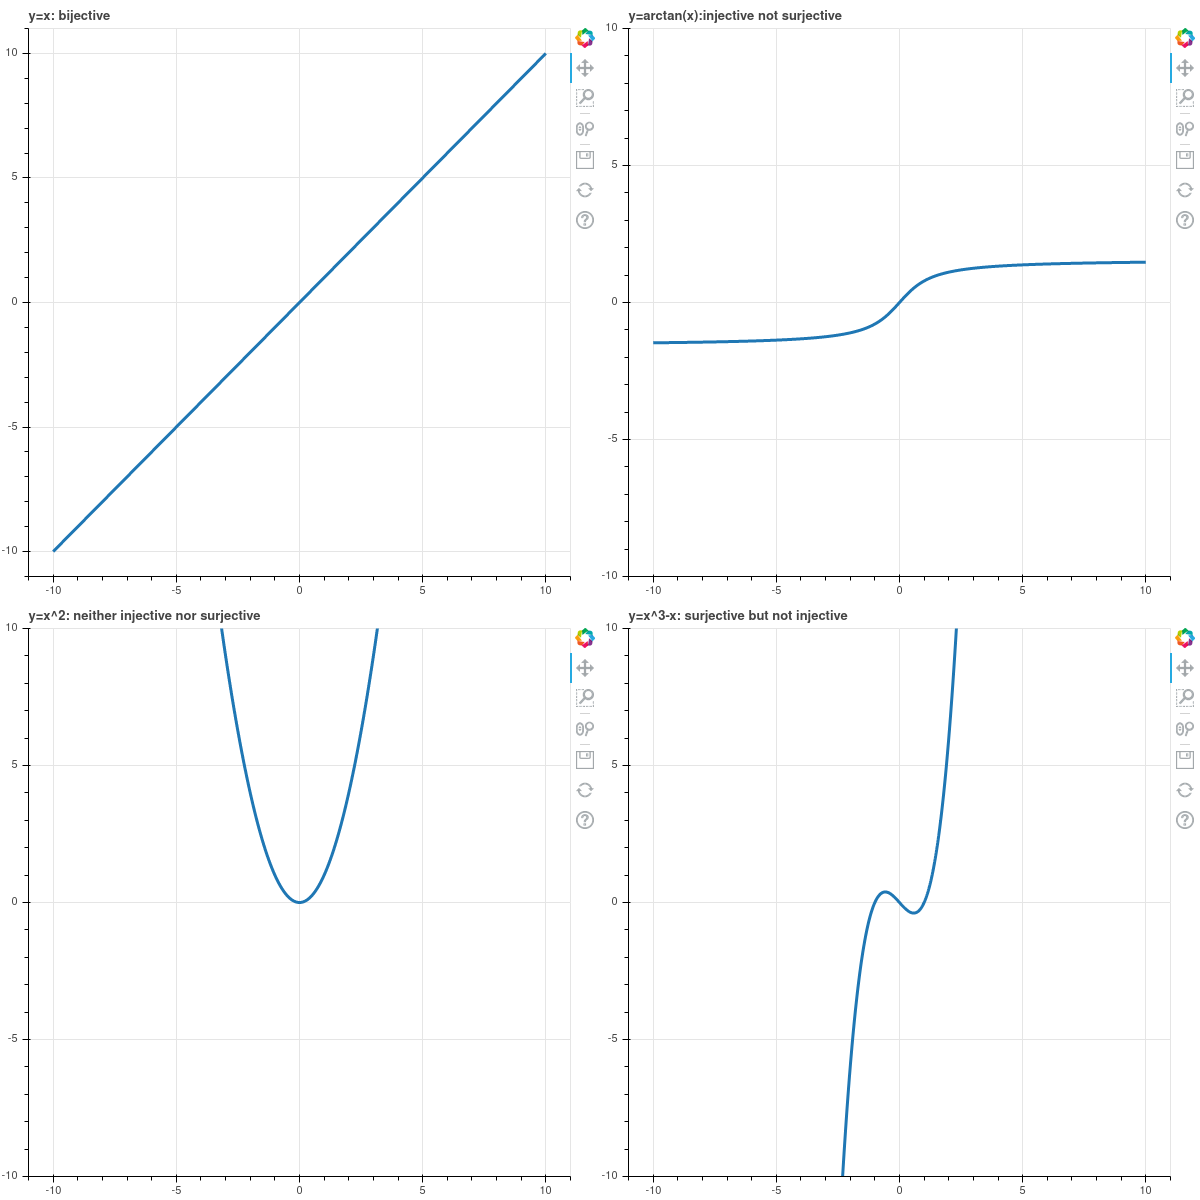
\includegraphics[width=1\textwidth,height=\textheight]{../png/injsurjbijexamples.png}

\vfill

\end{document}
